\documentclass{report}
% Include all project wide packages here.
\usepackage{fullpage}
\usepackage[style=ieee]{biblatex}
\usepackage[dutch]{babel}

\renewcommand{\familydefault}{\sfdefault}

\setmainfont[Ligatures=TeX]{Myriad Pro}
\setmathfont{Asana Math}
\setmonofont{Lucida Console}

\usepackage{titlesec, blindtext, color}
\definecolor{gray75}{gray}{0.75}
\newcommand{\hsp}{\hspace{20pt}}
\titleformat{\chapter}[hang]{\Huge\bfseries}{\thechapter\hsp\textcolor{gray75}{|}\hsp}{0pt}{\Huge\bfseries}
\renewcommand{\familydefault}{\sfdefault}
\renewcommand{\arraystretch}{1.2}
\setlength\parindent{0pt}

%For code listings
\definecolor{black}{rgb}{0,0,0}
\definecolor{browntags}{rgb}{0.65,0.1,0.1}
\definecolor{bluestrings}{rgb}{0,0,1}
\definecolor{graycomments}{rgb}{0.4,0.4,0.4}
\definecolor{redkeywords}{rgb}{1,0,0}
\definecolor{bluekeywords}{rgb}{0.13,0.13,0.8}
\definecolor{greencomments}{rgb}{0,0.5,0}
\definecolor{redstrings}{rgb}{0.9,0,0}
\definecolor{purpleidentifiers}{rgb}{0.01,0,0.01}


\lstdefinestyle{csharp}{
language=[Sharp]C,
showspaces=false,
showtabs=false,
breaklines=true,
showstringspaces=false,
breakatwhitespace=true,
escapeinside={(*@}{@*)},
columns=fullflexible,
commentstyle=\color{greencomments},
keywordstyle=\color{bluekeywords}\bfseries,
stringstyle=\color{redstrings},
identifierstyle=\color{purpleidentifiers},
basicstyle=\ttfamily\small}

\lstdefinestyle{c}{
language=C,
showspaces=false,
showtabs=false,
breaklines=true,
showstringspaces=false,
breakatwhitespace=true,
escapeinside={(*@}{@*)},
columns=fullflexible,
commentstyle=\color{greencomments},
keywordstyle=\color{bluekeywords}\bfseries,
stringstyle=\color{bluestrings},
identifierstyle=\color{purpleidentifiers}
}

\lstdefinestyle{vhdl}{
language=VHDL,
showspaces=false,
showtabs=false,
breaklines=true,
showstringspaces=false,
breakatwhitespace=true,
escapeinside={(*@}{@*)},
columns=fullflexible,
commentstyle=\color{greencomments},
keywordstyle=\color{bluekeywords}\bfseries,
stringstyle=\color{redstrings},
identifierstyle=\color{purpleidentifiers}
}

\lstdefinestyle{xaml}{
language=XML,
showspaces=false,
showtabs=false,
breaklines=true,
showstringspaces=false,
breakatwhitespace=true,
escapeinside={(*@}{@*)},
columns=fullflexible,
commentstyle=\color{greencomments},
keywordstyle=\color{redkeywords},
stringstyle=\color{bluestrings},
tagstyle=\color{browntags},
morestring=[b]",
  morecomment=[s]{<?}{?>},
  morekeywords={xmlns,version,typex:AsyncRecords,x:Arguments,x:Boolean,x:Byte,x:Char,x:Class,x:ClassAttributes,x:ClassModifier,x:Code,x:ConnectionId,x:Decimal,x:Double,x:FactoryMethod,x:FieldModifier,x:Int16,x:Int32,x:Int64,x:Key,x:Members,x:Name,x:Object,x:Property,x:Shared,x:Single,x:String,x:Subclass,x:SynchronousMode,x:TimeSpan,x:TypeArguments,x:Uid,x:Uri,x:XData,Grid.Column,Grid.ColumnSpan,Click,ClipToBounds,Content,DropDownOpened,FontSize,Foreground,Header,Height,HorizontalAlignment,HorizontalContentAlignment,IsCancel,IsDefault,IsEnabled,IsSelected,Margin,MinHeight,MinWidth,Padding,SnapsToDevicePixels,Target,TextWrapping,Title,VerticalAlignment,VerticalContentAlignment,Width,WindowStartupLocation,Binding,Mode,OneWay,xmlns:x}
}

%defaults
\lstset{
basicstyle=\ttfamily\small,
extendedchars=false,
numbers=left,
numberstyle=\ttfamily\tiny,
stepnumber=1,
tabsize=4,
numbersep=5pt
}
\addbibresource{../../library/bibliography.bib}
\begin{document}
\chapter{Resultaten en Discussie}
Er zijn drie verschillende metingen verricht, kalibratiemeting, onbekende afstandsmeting en de lineariteitsmeting. Deze metingen zijn drie keer gedaan en dus zijn de meetresultaten ook drie keer weergeven en geanalyseerd.
\section{Kalibratie}
Hieronder zijn de meetresultaten van de eerste kalibratiemeting te zien. Bij deze meting is het de bedoeling dat deze 10 keer wordt uitgevoerd, maar bij 1 groepje is de opdracht verkeerd ge\"interpreteerd en is de meting maar vijf keer uitgevoerd.\\

Als we de functies \label{eq:vel}, \ref{eq:avgTime},  \ref{eq:avgVel},  \ref{eq:standaardDev},  \ref{eq:timeError} en  \ref{eq:velError} op de meetresultaten (Tabel \ref{tab:measurementsCalib}) loslaten krijgen we de waarden als in Tabel \ref{tab:resCali}. De snelheid wijkt vooral bij Robin \& Erwin af dit komt door dat zij een andere robot gebruikt hebben.\\

In Figuur \ref{fig:measureGraph} zijn de metingen voor de kalibratie afgebeeld. De metingen RE (Robin \& Erwin) liggen vrij ver van de andere af omdat die metingen gedaan zijn met een andere robot, ook hadden dit 10 meetpunten moeten zijn.

\begin{figure}[H]
	\centering
	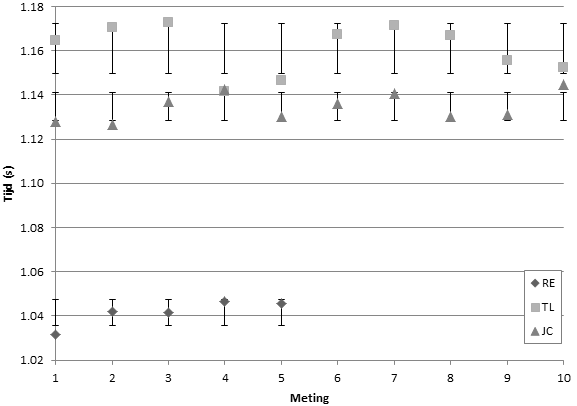
\includegraphics[width=0.7\textwidth]{kalibratie}
	\caption{De meetresultaten in een diagram, de foutbalken geven één standaarddeviatie aan.}
	\label{fig:measureGraph}
\end{figure}

\begin{table}
	\centering
	\caption{Meetresulataten kalibratie}
	\label{tab:measurementsCalib}
	\begin{subtable}[H]{0.30\textwidth}
		\centering
		\subcaption{Robin en Erwin}
			\begin{tabular}{| l| c|}
		\hline
		   Meting \# & t (s) \\
		\hline
		   1& 1.031 \\
		\hline
		   2& 1.042 \\
		\hline
		   3& 1.042 \\
		\hline
		   4& 1.046 \\
		\hline
		   5& 1.045 \\
		\hline
		\end{tabular}
	\end{subtable}
	\quad
	\begin{subtable}[H]{0.30\textwidth}
		\centering
		\subcaption{Joris en Chy}
		\begin{tabular}{| l| c|}
		\hline
		   Meting \# & t (s) \\
		\hline
		   1& 1.128\\
		\hline
		   2& 1.127\\
		\hline
		   3& 1.137\\
		\hline
		  4& 1.142\\
		\hline
		   5& 1.130 \\
		\hline
		   6& 1.136\\
		\hline
		   7& 1.140\\
		\hline
		   8& 1.130\\
		\hline
		   9& 1.131\\
		\hline
		   10& 1.145 \\
		\hline
		\end{tabular}
	\end{subtable}
	\quad
	\begin{subtable}[H]{0.30\textwidth}
		\centering
		\subcaption{Luc en Tijmen}
		\begin{tabular}{| l| c|}
		\hline
		   Meting \# & t(s) \\
		\hline
		   1& 1.170 \\
		\hline
		   2& 1.173 \\
		\hline
		   3& 1.142 \\
		\hline
		   4& 1.146 \\
		\hline
		   5& 1.164 \\
		\hline
		   6& 1.167 \\
		\hline
		   7& 1.171 \\
		\hline
		   8& 1.167\\
		\hline
		   9& 1.156\\
		\hline
		   10& 1.152\\
		\hline
		\end{tabular}
	\end{subtable}
\end{table}

\begin{table}
	\centering
	\caption{Eigenschappen Robot}
	\label{tab:resCali}
	\begin{subtable}[b]{0.30\textwidth}
		\centering
		\subcaption{Robin en Erwin}
		\begin{tabular}{| l| c|}
		\hline
			Naam & Waarde \\
		\hline
			$t_{gem}$ & 1.041 s \\
		\hline
			$v_{gem}$ & 0.0960 m/s \\
		\hline
			$s_{onb.}$ & 0.242 m \\
		\hline		  
		   $\sigma(t_{gem})$ & $ 5.3 \cdot 10^-3 \mathrm{s}$  \\
		\hline
		   $\sigma(v_{gem})$ & $0.684 \cdot 10^-3  \mathrm{ ^m/_s}$ \\
		\hline
		$\sigma(s_{onb})$ & $0.874 \cdot 10^-3 \mathrm{m}$ \\
		\hline
		\end{tabular}
	\end{subtable}
	\quad
	\begin{subtable}[b]{0.30\textwidth}
		\centering
		\subcaption{Joris en Chy}
		\begin{tabular}{| l| c|}
		\hline
		   Naam & Waarde \\
		\hline
		   $t_{gem}$ & 1.135 s \\
		\hline
		   $v_{gem}$ & 0.0881 m/s \\
		\hline
		$s_{onb.}$ & 0.240 m \\
		\hline		  
		   $\sigma(t_{gem})$ & $5.9 \cdot 10^-3 \mathrm{s}$  \\
		\hline
		   $\sigma(v_{gem})$ & $0.638 \cdot 10^-3  \mathrm{ ^m/_s}$ \\
		\hline
		$\sigma(s_{onb})$ &$ 0.894 \cdot 10^-3 \mathrm{m}$ \\
		\hline
		\end{tabular}
	\end{subtable}
	\quad
	\begin{subtable}[b]{0.30\textwidth}
		\centering
		\subcaption{Luc en Tijmen}
		\begin{tabular}{| l| c|}
		\hline
		   Naam & Waarde \\
		\hline
		   $t_{gem}$ & 1.161 s \\
		\hline
		   $v_{gem}$ & 0.0861 cm/s \\
		\hline
			$s_{onb.}$ & 0.235 m \\
		\hline		  
		   $\sigma(t_{gem})$ & $11 \cdot 10^-3\mathrm{s}$  \\
		\hline
		   $\sigma(v_{gem})$ & $0.897 \cdot 10^-3 \mathrm{ ^m/_s}$ \\
		\hline
		$\sigma(s_{onb})$ & $1.39 \cdot 10^-3 \mathrm{m}$ \\
		\hline
		\end{tabular}
	\end{subtable}
\end{table}

\section{Onbekende afstand}

In Tabel \ref{tab:resExtraUnknownD} zijn de meetresultaten te zien van de onbekende afstandsmeting. Om de snelheid te kunnen bepalen moet er een afstand bekend zijn. Deze afstand is gemeten met een liniaal en deze is $0.234 \pm 0.0005\mathrm{m}$. De met de robot gemeten afstand zijn strijdig voor de metingen RE en JC omdat voor deze metingen niet voldaan wordt aan de voorwaarde als in Formule \ref{eq:strijdigheid}, de meting van Luc en Tijmen is niet strijdig. Deze strijdigheid komt waarschijnlijk omdat de robot in een boog reed en dat daardoor de gemeten afstanden allemaal hoger uitvallen.


\begin{table}
	\centering
	\caption{De resultaten van de onbekende afstandsmetingen en de lineairiteitsmetingen.}

	\begin{subtable}[b]{0.33\linewidth}
		\centering
		\subcaption{Onbekende afstand}
		\label{tab:resExtraUnknownD}
		\begin{tabular}{| l| c|}
		\hline
		  Meting \#  & t (s)\\
		\hline
		  R\&E & 2.526 \\
		\hline
		J\&C & 2.664 \\
		\hline
		L\&T & 2.741 \\
		\hline
		 \end{tabular}
	\end{subtable}
	\begin{subtable}[b]{0.66\linewidth}
		\centering
		\subcaption{Lineairiteit}
		\label{tab:resExtraLin}
		\begin{tabular}{| l| c| c| c| c| c|}
		\hline
		  Meting \# & $t_{5cm} (s)$ & $t_{10cm} (s)$ & $t_{15cm} (s)$ & $t_{20cm} (s)$ & $t_{25cm} (s)$\\
		\hline
		  R\&E & 0.542 & 1.092 & 1.638 & 2.218 & 2.728 \\
		\hline
		J\&C & 0.575 & 1.140 & 1.732 & 2.330 & 2.854 \\
		\hline
		L\&T & 0.584 & 1.177 & 1.789 & 2.375 & 2.955 \\
		\hline
		 \end{tabular}
	\end{subtable}
\end{table}

\section{Lineariteit}
\subsection*{Meting 1}
In Tabel \ref{tab:resExtraLin} zijn de meetresultaten te zien van de lineariteitsmeting. Doormiddel van de meetresultaten en de afstand is de gemiddelde snelheid uitgerekend. De grafiek in Figuur \ref{fig:linGraph} geeft een duidelijk beeld van de metingen ten opzichte van de uitgerekende gemiddelde snelheid. Het is te zien dat er voor de afwijking in de rijrichting van de robot, deze rijdt in een cirkel, de afwijking in de gemeten tijd groter wordt naarmate de afstand tussen de lijnen toeneemt.

\begin{figure}[H]
	\centering
	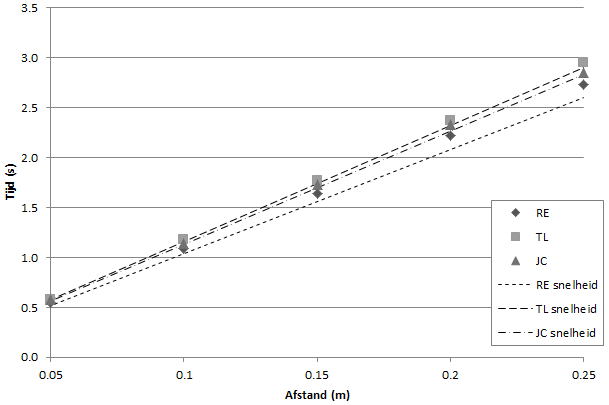
\includegraphics[width=0.7\textwidth]{lineairiteit}
	\caption{De lineairiteitsmetingen en de uitgerekende snelheid van de kalibratie in 1 grafiek.}
	\label{fig:linGraph}
\end{figure}

\newpage
\chapter{Conclusie}
Het meetresultaat van dit meetrapport is goed te gebruiken in de rest van ons project. Dit is mede te danken aan de hoge kwaliteit van de meetresultaten. De onzekerheid en de afwijkingen zijn erg klein bij alle metingen die zijn verricht. De gemiddelde snelheid van de robot is ongeveer 9,6 cm/s. Bij de lineariteitsmeting was de gemiddelde snelheid vrijwel onafhankelijk van de afstand, en dus is de afstandsmeter van de robot erg lineair. Tijdens het rijden maakt de robot een bocht met een radius van ongeveer 80 cm. Hiermee moet rekening gehouden worden bij het programmeren van de robot. Het feit dat de afstandsmeter van de robot erg lineair is, is een gunstige conclusie voor ons project.
\end{document}



\end{document}